\documentclass[
% opciók nélkül: egyoldalas nyomtatás, elektronikus verzió
% twoside,     % kétoldalas nyomtatás
% tocnopagenum,% oldalszámozás a tartalomjegyzék után kezdődik
]{thesis-ekf}
\usepackage[T1]{fontenc}
\PassOptionsToPackage{defaults=hu-min}{magyar.ldf}
\usepackage[magyar]{babel}
\usepackage{mathtools,amssymb,amsthm,pdfpages}
\usepackage{enumitem}
\footnotestyle{rule=fourth}

\newtheorem{tetel}{Tétel}[chapter]
\theoremstyle{definition}
\newtheorem{definicio}[tetel]{Definíció}
\theoremstyle{remark}
\newtheorem{megjegyzes}[tetel]{Megjegyzés}

\begin{document}
	\institute{Matematikai és Informatikai Intézet}
	\title{A kommunikációs gráfok modelljeinek vizsgálata Python programozási nyelvvel}
	\author{Mohai Ferenc\\programtervező informatikus BSc}
	\supervisor{Dr.~Kusper Gábor\\egyetemi docens}
	\city{Eger}
	\date{2022}
	
	\maketitle
	\tableofcontents
	
	\chapter*{Bevezetés}
	\addcontentsline{toc}{chapter}{Bevezetés}
	A szakdolgozati szemináriumon, amikor hallottam Kusper Gábor tanár úr magyarázatát a kutatásról, annak eredményeiről, céljáról, felhasználásáról. és már akkor nagyon megtetszett a téma. A SAT megoldó széles körű felhasználásáról beszélgettünk. Korábbi előadásokon, gyakorlatokon is voltak tanáraim, akik ezt a témát felvetették, és már akkoriban meghozták a kedvemet hozzá. Amikor választanom kellett, nem volt nagy kérdés, hogy ez egy számomra érdekes téma, amivel szívesen dolgozok, és lehetőséget ad a fejlődésre.

	Szaktársammal, Rajna Franciskával csak mi ketten érdeklődtünk ebben a témában, úgyhogy mindenki örömmel beszélte meg a részleteket és közös megegyezéssel találtuk ki melyik ágát dolgozza ki a témának. Pozitív és energikus első benyomás után örömmel kezdtünk a munkának. Bíró Csaba és Balla Tamás tanár urakkal dolgoztunk a témával kapcsolatos házi TDK-hoz hasonló előadásokon és kutatásokon (\cite[ICAI2020, AM2020]{am}) vettünk részt. Az egyik alkalommal egy plakátot is készítettünk, ezekkel megalapozva egy lendületes kezdést.
	
	Megbeszéltük hol szorul fejlesztésre a SAT megoldó, amin tudok programozással javítani. Valamint a korábbi általuk írt angol nyelvű szakirodalmakkal elsajátíthatom az elméleti hátteret, felzárkózhatok a jelenlegi helyzethez és ezeken dolgozva könnyedén belerázódjak a szakdolgozatom megfogalmazásába. Így kezdtem el a munkámat.
	
	\chapter{Alap fogalmak}
	
	A munkámat azzal kezdtem, hogy szakirodalmakat olvastam, fordítottam és értelmeztem, amiket korábban témavezetőim írtak [RÉSZLETEZD az alapokat SZAKIRODALOM]. Anyagot gyűjtöttem és dolgoztam fel a SAT megoldókról. Ezekben megjelentek különböző fogalmak, mint a tautológia [RÉSZLETEZD az alapokat alfejezetben SZAKIRODALOM FOGALMAI] cnf, és dnf, valamint programozási nyelvek, mint a Python [RÉSZLETEZD az alapokat PYTHON] és a Wolfram Alpha [RÉSZLETEZD az alapokat WOLFRAM ALPHA].
	
	\section{Szakirodalom}
	Szakirodalom fogalmai, definíciói:
	
	\begin{definicio}
		Atomi formula, röviden atom:  Azt mondjuk, hogy egy szimbólum atomi formula, vagy atom, akkor és csak akkor, ha egy kifejezést jelöl. Ilyen atomok, az igaz és hamis ítéletváltozók. Szimbólumuk általában az \emph{I} és \emph{H} betűk magyarul, de szoktuk használni az angol megfelelőjét is a \emph{T} és \emph{F} betűket.
	\end{definicio}
	\begin{definicio}
		Literál: Azt mondjuk, hogy egy szimbólum literál, akkor és csak akkor, ha egy atom, vagy annak negáltja.
	\end{definicio}
	\begin{definicio}		
		Jól formázott formula, röviden formula: Azt mondjuk, hogy egy szimbólum sorozat jól formázott formula, vagy formula, akkor és csak akkor, ha F formula a következő alakok egyikében van:
		\begin{enumerate}[label=\textit{(\alph*)}]
			\item A, ahol A egy atom;
			\item $ \neg A $, ahol A egy formula;
			\item $ (A \wedge B) $, ahol A és B formulák;
			\item $ (A \vee B) $, ahol A és B formulák;
			\item $ (A \implies B) $, ahol A és B formulák;
			\item $ (A \Leftrightarrow B) $, ahol A és B formulák.
		\end{enumerate}
		Minden formula a fenti esetek véges sokszori alkalmazásával áll elő.
	\end{definicio}
	\begin{definicio}
		Formula: Adott ítéletváltozónak egy véges, nem üres V halmaza.
		\begin{enumerate}
			\item Ítéletváltozó: ha $ A\in V $, akkor A formula.
			\item Negáció: ha A formula, akkor $\neg A $ is formula.
		\end{enumerate}
	\end{definicio}
	\begin{definicio}
		Klóz, angolul clause: Azt mondjuk, hogy egy formula klóz, akkor és csak akkor, ha adott literáloknak és formális összekötőknek egy véges, nem üres, egynél több elemű W halmaza.
		\begin{enumerate}
			\item pozitív literál: ha $ B\in W $, és B egy pozitív literál.
			\item negatív literál: ha B pozitív literál, akkor $\neg B $ negatív literál.
			\item és formális összekötő: ha $ B \wedge \neg B $, akkor $\wedge$ egy és formális összekötő.
			\item vagy formális összekötő: ha $ B \vee \neg B $, akkor $\vee$ egy vagy formális összekötő.
		\end{enumerate}	
	\end{definicio}
	\begin{megjegyzes}
		Létezik konjunktív és diszjunktív klóz is. Ezeket később részletezem.
		Diszjunktív klóz: Azt mondjuk, hogy $ l_{i} $ szimbólumok egy klózt alkotnak, akkor és csak akkor, ha minden $ l_{i} $ literál: $ l_{1}\vee\dots\vee l_{n} $
		Konjunktív klóz: Azt mondjuk, hogy $ l_{i} $ szimbólumok egy klózt alkotnak, akkor és csak akkor, ha minden $ l_{i} $ literál: $ l_{1}\wedge\dots\wedge l_{n} $
	\end{megjegyzes}
	\begin{definicio}
		Implikáció: Azt mondjuk hogy formális összekötő implikáció, akkor és csak akkor, ha mindkét oldalán van egy literál, és egy harmadik literált állít elő a kettő értékéből, oly módon, hogy az összes bal oldali értékből pozitív literált állít elő, kivéve, ha a bal oldalán pozitív, a jobb oldalán negatív literál van.
		Mivel a negatív értékből nem következik a pozitív érték. Jelölése: $ A \implies B $
	\end{definicio}
	\begin{definicio}
		Ekvivalencia: Azt mondjuk, hogy formális összekötő ekvivalencia, akkor és csak akkor, ha mindkét oldalán van egy literál, és egy harmadik literált állít elő a kettő értékéből, oly módon, hogy ha mindkét oldalán ugyan az a pólusú literál van, akkor pozitív literált állít elő, kivéve, ha eltérnek a pólusok.
	\end{definicio}
	\begin{megjegyzes}
		Pólus alatt a negatív vagy pozitív jelzőt értjük.
	\end{megjegyzes}
	\begin{definicio}
		Konjukció: Azt mondjuk, hogy formális összekötő konjukció, akkor és csak akkor, ha mindkét oldalán van egy literál, és egy harmadik literált állít elő a kettő értékéből, oly módon, hogy ha mindkét oldalán pozitív literál van, akkor és csak akkor pozitív literált állít elő, különben negatív literált. Jele: $\wedge$
	\end{definicio}
	\begin{definicio}
		Diszjunkció: Azt mondjuk, hogy formális összekötő diszjunkció, akkor és csak akkor, ha mindkét oldalán van egy literál, és egy harmadik literált állít elő a kettő értékéből, oly módon, hogy ha mindkét oldalán negatív literál van, akkor negatív literált állít elő, különben pozitív literált. Jele: $\vee$
	\end{definicio}
	\begin{definicio} % megjegyzésbe kiemelni az angol megfelelőket? CNF DNF
		Konjunktív normál forma, röviden KNF, angolul conjunctive normal form, mint CNF: Azt mondjuk, hogy logikai formula konjunktív normál forma, akkor és csak akkor, ha egy vagy több klózt egymáshoz kötünk konjunkcióval.
	\end{definicio}
	\begin{definicio}
		Diszjunktív normál forma, röviden DNF, angolul disjunctive normal form, mint DNF: Azt mondjuk, hogy logikai formula diszjunktív normál forma, akkor és csak akkor, ha egy vagy több klózt egymáshoz kötünk diszjunkcióval.
	\end{definicio}
	\begin{definicio}
		Interpretáció: Adott ítéletváltozóknak egy véges sok, nem üres V halmaza.
		Azt mondjuk, hogy a J hozzárendelés az F formula egy interpretációja, akkor és csak akkor, ha F minden atomjához vagy az igaz, vagy a hamis értéket rendeljük, de csak az egyiket.
	\end{definicio}
	\begin{definicio}
		Logikai törvény, más néven tautológia: Azt mondjuk, hogy az F formula logikai törvény, vagy tautológia, akkor és csak akkor, ha F minden interpretációjában igaz.
	\end{definicio}
	\begin{definicio}
		Logikai ellent mondás, angolul contradiction, unsatisfiable: Azt mondjuk, hogy az F formula logikai ellentmondás, akkor és csak akkor, ha F minden interpretációjában hamis.
	\end{definicio}
	\begin{definicio}
		Kielégíthető, angolul satisfiable: Azt mondjuk, hogy az F formula kielégíthető, akkor és csak akkor, ha F legalább egy interpretációjában igaz.
	\end{definicio}
	\begin{definicio}
		Hamissá tehető, angolul falseable: Azt mondjuk, hogy az F formula hamissá tehető, akkor és csak akkor, ha F legalább egy interpretációjában hamis. 
	\end{definicio}
	\begin{megjegyzes}
		Kielégítő ellentéte a logikai ellentmondás, mivel ha valami nem kielégíthető, akkor abból következik, hogy logikai ellentmondás.
		Hamissá tehető ellentéte a logikai törvény, mivel ha valami nem hamissá tehető, akkor abból következik, hogy logikai törvény.
	\end{megjegyzes}


	\begin{itemize}	
		\item Igazság tábla: Oszloponként tartalmazza az összes atomot, ami a formulánkban van, és az utolsó oszlopban a formulát is. Soronként minden atomhoz értéket rendel (minden lehetséges sorrendben), és a formulába behelyettesítve kiszámítja a formula értékét. Az eredményét az utolsó oszlopban láthatjuk.
		\item Logikai törvény, tautológia: Ezek segítségével felírhatunk olyan formulákat, és igazság táblákat, amelyek minden lehetséges esetre igaz értéket adnak eredményül.
	\end{itemize}

	részletet beilleszteni a szakirodalom fordításaimból.


	\section{A Python programozási nyelvről}
	részletezés
	\cite[102.~oldal]{Fazekas}
	
	szöveg
	\cite{Fazekas,Tomacs}
	
	\begin{tetel}
		Tétel szövege.
	\end{tetel}
	
	\begin{proof}
		Bizonyítás szövege.
	\end{proof}
	

	

	
	\chapter*{Összegzés}
	\addcontentsline{toc}{chapter}{Összegzés}

	
	\begin{thebibliography}{2}
		\addcontentsline{toc}{chapter}{\bibname}
		\bibitem{am}
		\textsc{ICAI2020, AM2020 - Agria Média}: ...
		\bibitem{Fazekas}
		\textsc{Fazekas István}: \emph{Valószínűségszámítás}, Debreceni Egyetem, Debrecen, 2004.
		\bibitem{Tomacs}
		\textsc{Tómács Tibor}: \emph{A valószínűségszámítás alapjai}, Líceum Kiadó, Eger, 2005.
	\end{thebibliography}
	
	% Aláírt, szkennelt nyilatkozat beillesztése a szakdolgozat végére
	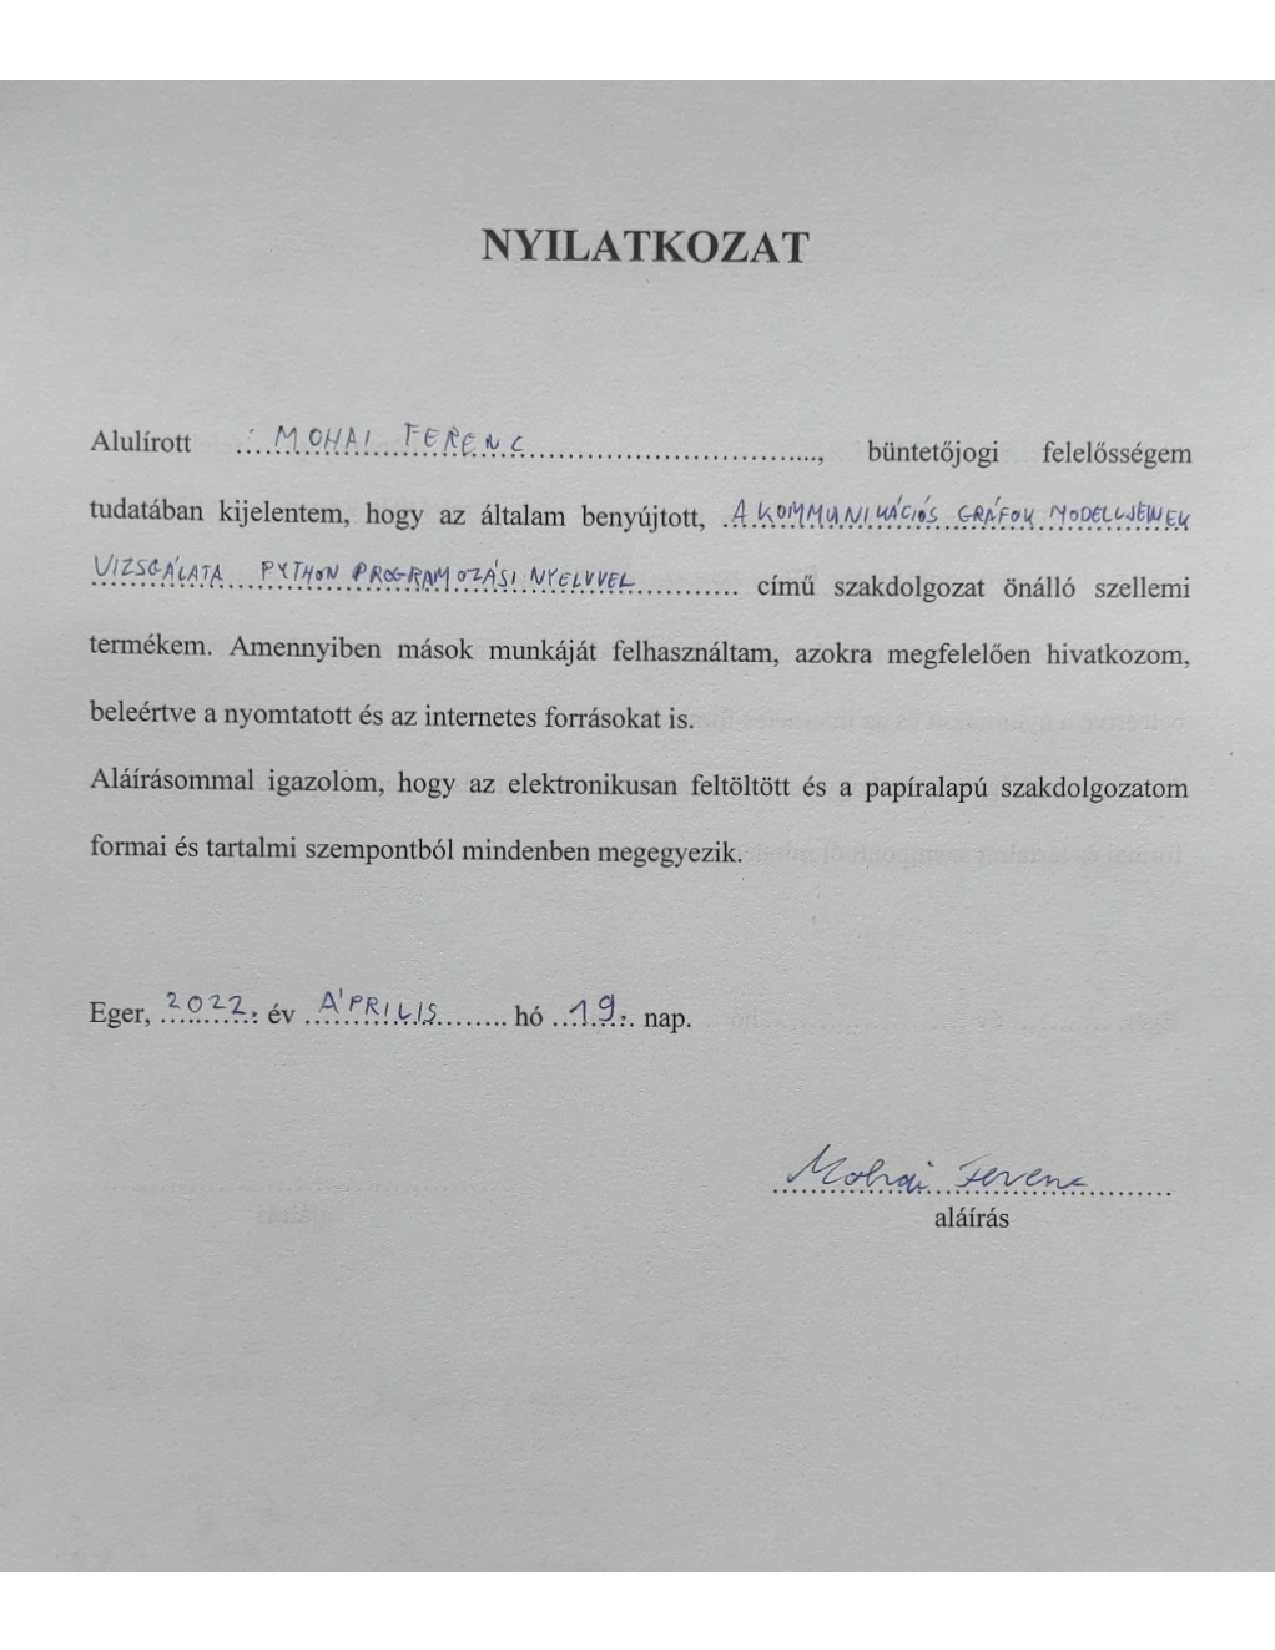
\includepdf[pagecommand={\thispagestyle{empty}}]{nyilatkozat.pdf}
\end{document}